\documentclass{article}

\usepackage{hyperref}       % hyperlinks
\usepackage{url}            % simple URL typesetting
\usepackage{amsfonts}       % blackboard math symbols
\usepackage{amsmath}
\usepackage{graphicx}

\usepackage[T1]{fontenc}
\usepackage[utf8]{inputenc}
\usepackage{tabularx,ragged2e,booktabs,caption}
\newcolumntype{C}[1]{>{\Centering}m{#1}}
\renewcommand\tabularxcolumn[1]{C{#1}}

% Used to change margins, I really don't like Latex...
% Got from here: https://stackoverflow.com/questions/1670463/latex-change-margins-of-only-a-few-pages
\newenvironment{changemargin}[2]{%
\begin{list}{}{%
\setlength{\topsep}{0pt}%
\setlength{\leftmargin}{#1}%
\setlength{\rightmargin}{#2}%
\setlength{\listparindent}{\parindent}%
\setlength{\itemindent}{\parindent}%
\setlength{\parsep}{\parskip}%
}%
\item[]}{\end{list}}

\title{CSE 151B Project Milestone Report}

\author{%
  Justin Allen
  \texttt{jballen@ucsd.edu}
}

\begin{document}

\maketitle

\section{Task Description and Exploratory Analysis}

\subsection{Task Description}

Our goal is to predict the future movement of a tracked car given information on its previous position and velocity, the positions and velocities of other objects near this car, and lane information. This problem is also known as Motion Forecasting, and is vital in the production of self driving cars.

We are given 5 seconds of training information on the positions and velocities of up to 60 objects in a single scene, as well as information on the lanes in the scene, sampled at 10HZ. We must use the first 19 time steps to predict the motion of a single agent car over the next 3 seconds (30 time steps). After training models, they are tested on a validation set containing only the first 19 time steps.

Note: all figures and tables are at the end of this paper.

\subsection{Data Analysis}

The training set consists of 205,942 samples, and the validation 3200. More information about the raw data can be found on my Kaggle discussion post here: \url{https://www.kaggle.com/c/cse151b-spring/discussion/233734}. 

Figure 1 shows the histograms for $x$ and $y$ value distributions in the dataset. Figure 2 shows the histogram of object speeds. Figure 3 shows a map of the coordinate space of the raw data with the lanes drawn in based on their centers and norms. 

From these two figures, we can see that the raw data (1) contains very large values, (2) tends to group up, and (3) has some notably large outliers. The position data tends to fall in certain groups corresponding to where there are lanes in the map. The velocity data is mostly grouped around 0, with a very small number of outliers. 

It may not be the best idea to use the data in its raw state, even if normalized, as it likely would not be able to generalize into different coordinate systems or different cities. So, we also create a modified training dataset. Instead of raw values, each value at each time step is changed to be the offset from the previous time step.

$$ X_{t, o, i} := X_{t, o, i} - X_{t, o, i} $$

Where $X$ is any of the p\_in, p\_out, ... for a given scene, $t$ is the time step from $2 \leq t \leq 19$, $o$ is the object in the scene ranging from $1 \leq o \leq 60$, and $i=0,1$ is the $x$ and $y$ coordinate. This cannot be applied to the first time step since there is no previous time step. We instead use this first time step as a measure of the offset from each object in the scene to the agent car. This has the side effect of setting the initial position of the agent car to (0, 0) for every scene.

$$ X_{1, o, i} = X_{1, o, i} - X_{1, 1, i} $$

This is applied to all of the p\_in, ... values. For lane center information, we only apply the offset from the agent car's initial position.

$$ L_{n, i} = L_{n, i} - P_{1, 1, i} $$

Where $L$ is the list of lane centers, $n$ is the index of the given lane in that list, and $P$ is the p\_in array. Nothing is done to alter the lane\_norm array as its values are already not dependant on the coordinate system. For both datasets, we take a maximum of 100 lanes, with any unused lanes being set to 0.

These alterations remove the need to rely on the coordinate system for information, and instead are only based on the agent car's initial position, and whatever measurement system the Argoverse dataset curators used (most likely a standard one like meters or feet). This also allows us to identify and deal with outliers more effectively. Figure 4 shows the histogram data for this new dataset, labeled the 'step' dataset.

Table 1 shows statistics on different sections of the dataset (all data and validation separately). Combined with the histogram information in Figure 4, we see that this 'step' dataset still has outliers, and these outliers are present even in the inputs of the validation set, implying they would likely be present in the outputs we are trying to predict as well. So, we must make sure to include the ability for our models to predict outliers if we wish to minimize our total RMSE on the validation set. This leads us to the next section of data normalization.

\subsection{Normalization}

We test multiple different normalization methods on the data with our models (Model descriptions in section 2). Let $X$ be a section of our data, $X'$ be the normalized data, $m$ be the minimum values in $x$ and $y$, $M$ the max values, $a$ the average/mean, and $s$ the standard deviation. We test the following normalization methods:\\\\

"noop": 'no-op' or 'no operation' - not normalizing the data at all\\\\
"linear": a min-max normalization - $X' = \frac{(X - m)}{M-m} * (V-v) - v$ where $V$ is the maximum value we want output, and $v$ the min. This normalizes our data linearly into the range $[v, V]$.\\\\
"standardize": standardize the data to have mean zero and standard deviation one - $X' = (X - a) / s$\\\\
"tanh": hyperbolic tangent of the data, used only in tests on neural networks - $X' = tanh(X)$\\\\
"std\_step": short for "standard step", a novel normalization function (at least, I couldn't find anything like it online. Most likely it's been done, or something similar, and I just don't know what to google). The intuition behind this function is as follows: most of the input 'step' data falls into a short range (for example, the "p\_step" values have standard deviation of ~[0.46, 0.57] over all data). However, we must be able to work with and output large outlier values, even if they are rare. So, we normalize the value within a small number (say, 2-3) of standard deviations to be within a small range (such as [-1, 1]). Then the remaining values are normalized into a slightly larger range on their own (say, [-2, -1] for values less than the standard deviation cutoff, and [1, 2] for values larger). This way, smaller but more common values are normalized in such a way that they barely change, and the larger outlier values are still workable into our models. For the cost of slightly lower fidelity on outliers, we gain far higher fidelity on more common values. This would likely not have much of an effect on models such as Random Forests or Decision Trees as they are not affected by the magnitudes of data, but might have an impact on neural networks trained with gradient descent as it doesn't need to have as exact of values to have a low RMSE. This is the best method I could think of that allows high fidelity on most of the data, while being able to better represent all outputs, and while restricting input to a specific range. The formula is

$$ S_{min} = a - ks, \; S_{max} = a + ks $$
$$ Z_{min} = min(S_{min} - s, m), \; Z_{max} = max(S_{max} + s, m) $$
$$ x' = \begin{cases} 
    (x - Z_{min}) / (S_{min} - Z_{min}) * (r - v) + v &\mbox{if } x < S_{min} \\
    (x - S_{max}) / (Z_{max} - S_{max}) * (V - R) + R &\mbox{if } x > S_{max} \\
    (x - S_{min}) / (S_{max} - S_{min}) * (R - r) + r &\mbox{otherwise}\\
    \end{cases}$$
\\
Where $S_{min}, S_{max}$ are the cutoffs in the non-normalized data where all values within the range $[S_{min}, S_{max}]$ are mapped with high fidelity and all values outside that range are mapped with low fidelity, $k$ is the number of standard deviations to use in each direction from the mean to determine $S_{min}, S_{max}$, $Z_{min}, Z_{max}$ are the lowest and highest values in the non-normalized data (or, in the event that $a-ks$ or $a + ks$ is smaller/larger than the minimum/maximum value in the non-normalized data, one standard deviation further away from $S_{min}, S_{max}$, and $[r, R]$ is the range on which to map the data within $[S_{min}, S_{max}]$, for any $x \in X, \; x' \in X'$.

\subsection{Extra Features}

We also test our models on including/excluding lane information, as well as giving information on the current speed of all objects in the scene. The speed is included mainly as a possible improvement to models such as random forests which (to my knowledge) can only approximate functions involving ratios/square roots.

\section{Machine Learning Models and Experiment Design}

This section is split into three main parts given the very original names of "initial", "secondary", and "final" tests. The goal of the initial tests is to try out a wide range of simpler machine learning techniques on a smaller section of the data to get an idea of what models might perform well, and on what sets of data and normalization functions. The secondary tests take those that performed the best in the initial tests and fiddles with the hyperparameters to find the best values. The final finish up any hyperparameter search. Hyperparameters were tuned using a grid-based search.

All models were trained on my personal computer with a 2080TI GPU, 64GB memory, and AMD Ryzen 9 3900X 12-core 24-thread CPU. Models were built using SKLearn and Keras with Tensorflow-gpu. All code can be found here: \url{https://github.com/GlorifiedStatistics/ArgoverseTracking}.

In order to actually make the predictions, all models output the full 60 values ($x$ and $y$ values over 30 time steps). I had thought about also testing models that only output one $x$, $y$ pair corresponding to the next time step, and then feeding that back in to the model with a sliding window to produce future time steps, however I feel this would have problems. I believe that any errors accrued during prediction would tend to stack and increase as the predictions continued for each scene. If the model made a mistake near the beginning of the output, then those mistakes would be carried over as input for the next time step predictions. However, when outputting all 60 values at once, any of them could potentially be wrong with the rest of them remaining correct.

\subsection{Initial Tests}

The initial tests consist of the SKLearn regression models: k nearest neighbors, linear regression, elastic net, kernel ridge, general linear model, SGD regression, passive aggressive regression, Gaussian process, decision tree, and random forest, and well as the Keras model MLP. For each of the SKLearn models, we train using 10,000 examples and test on another 10,000 (from the training data), and test all combinations of data\_type ('raw' or 'step'), normalization function or 'norm\_func' ('noop', 'linear', 'standardize', 'std\_step'), and a few major hyperparameters (the $k$ in k nearest neighbors, the $p$ for the power of the general linear model, and the loss/penalty for the SGD regressor). The SKLearn models were only given 10,000 examples to train on due to time/memory constraints. Any other kwargs not mentioned were left to their SKLearn default values.

The MLP was given all data to train on with 20\% being set aside for testing, and was tested on some combinations of data\_type, norm\_func, and activation function. It had 4 hidden layers, used batch normalization (this was necessary for any MLP model to function), and did not use any dropout or regularization. MLP layer sizes decreased logarithmically from the input to the output size. 

None of the SKLearn tests included any lane information or extra features to help with speed of training, however the MLP models did include this information as it barely increased training time. As such, it might not be fair to compare these models just yet. 

Table 2 shows the top two best performing models from each category, as well as any other notable models. As is often the case in my experience, the random forest model performed the best of all SKLearn models with a RMSE of only 3.03 using the 'step' data and the 'standardize' normalization function (although, the 'noop' function was a close second, and the other functions were also pretty similar). The best MLP model used the 'step' data, and the 'tanh' normalization function with a tanh activation and achieved RMSE of 3.18. Most models had some combination of hyperparameters that produced acceptable results, except for the linear regression models which failed completely. Most models performed better on the 'step' data than the 'raw' data, and also performed worse using the 'std\_step' normalization function (oh well, at least I'm 1 for 2 of my ideas working). I cannot think of any reason why 'std\_step' normalization would perform so much worse on all models, including the MLP's, other than I have an error in the math or a bug in the code. I think it should at least be as effective as or better than the 'tanh' normalization since it should have similar fidelity on values close to 0, and better fidelity on the larger values due to the fact that 'tanh' approaches its asymptote rather quickly. If you reading this have any ideas, please let me know!

Armed with this information, we can now begin the secondary tests.

\subsection{Secondary Tests}

For these tests, we take the best models from the initial tests, and fiddle with their hyperparameters even more to attempt better results. We still wish to only use 10,000 examples on the SKLearn models, so the only hyperparameters to change would be the random forests' 'n\_estimators' and 'max\_depth'. In my experience, I find these will have little effect so long as 'n\_estimators' stays over 100 or so, and 'max\_depth' over 20, but it is still interesting and informative to test. We also have to ability to test a new model: the AdaBoostModel. I waited until now so we knew what initial hyperparameters to use, as training the AdaBoost model takes a very long time, and it relies on a decision tree as the underlying model. MLP models were tested using different values of dropout (0, 0.2, 0.4, 0.8) and different kernel regularizations (none, l1, l2, l1\_l2). MLP layer sizes decreased logarithmically from the input to the output size. We also test the inclusion and exclusion of lane information and the extra features for the random forest models.

These tests were done using values of other hyperparameters that performed well in the initial tests. The goal of this set of tests is not to find the very best hyperparameters, but instead to search a different set of hyperparameters to see their efficacy, as a full grid-based search of all hyperparameters would take far too long.

Table 3 shows some of the top models of each tested type (random forest, AdaBoost, and MLP), as well as any other notable models. The AdaBoost models seem to take the lead finally breaking past the 3.0 RMSE barrier, with the best reaching 2.93. Max\_depth and n\_estimators had a very small, but noticeable effect on the random forest's performance. To my surprise, the lane and extra feature information seemed to not make much of a difference on the random forest's performance either. For the MLP's dropout seemed to have little effect when it was small ($\leq 0.4$) and noticeably worsened performance when it was larger. All forms of kernel regularization also seemed to worsen performance. This makes sense as so far, we were not having any problem with overfitting, partially thanks to our necessary batch normalization. This does mean that if we are facing overfitting in the future, a small dropout might be able to improve performance as well. Finally, the best number of hidden layers tested was 5 (not including the output layer, so 6 layers in total). More testing might need to be done on differently sized layers, and more layers in total as 5 was the max tested.

\subsection{Final Tests}

These tests only involve neural network models as the SKLearn models have been tested thoroughly. Here, our goal is to find the best MLP model in a reasonable amount of time. Also, we intend to test some basic RNN architectures armed with the knowledge of effective MLP model hyperparameters.

Our RNN's consist of one RNN cell (either SimpleRNN, LSTM, or GRU) which takes the full input. Each time step in the dataset is considered one time step in the network, and the lane information if present is copied for all time steps. After going through all 19 time steps of input, the RNN state is passed along to some number of fully connected layers until reaching an output of 60 values. The goal is to test a simple RNN architecture to see if more complex architectures are warranted. RNN's using lane information were only given 50,000 examples due to memory limitations.

Table 4 shows all of the models tested. We see that the most effective MLP has 6 hidden layers with an RMSE of about 3.02, less than that of the 5 hidden layer model with the same kwargs in the secondary tests which had an error of about 3.08. The RNN models show that the best rnn\_type is an LSTM, that the number of neurons in the RNN cell does not effect accuracy too much, and that the RNN works better without the copied lane information. I do not believe the smaller training set size played a major role in this decrease of accuracy, and was instead mostly caused by too many inputs with lane information. The RNN has the lowest RMSE of any neural network tested, meaning more complex model types should be tested. More on this in section 3 Future Work.

\section{Experiment Results and Future Work}

Now that we have a good idea of what hyperparameters perform best, all model types that have achieved an RMSE error of $<4$ are tested with their best hyperparameters, and their predictions are saved and uploaded to Kaggle. Then, I talk about possible future work to achieve higher accuracies before the end of the semester.

\subsection{Best Models Results}

Table 5 shows the best models and their performance on both the test set, and the Kaggle validation set. All models were given all of the training data except for the KernelRidge, General Linear, and AdaBoost models due to memory. Early stopping was implemented in the neural network models where the epoch with the best RMSE on the test set is used for validation predictions. The AdaBoost model performed the best on Kaggle with a validation RMSE of about 2.377. I am currently \#1 on the class leaderboard (as of May 4th, 4PM).

\subsection{Model Performance Analysis}

Figure 5 shows the RMSE over time for the neural network models. The models are able to train very quickly (within about 5 epochs), then converge. Far larger epochs than 75 were tested with similar results. The RNNModel had its lowest RMSE's early on (around 10 epochs), showing it started to slightly overfit as time went on.

Figure 6 shows predicted vs. ground truth paths of agent cars in the test set for the best performing model, AdaBoostModel. The model is judged on its minimum, median, mean, and max stats for FDE, ADE, and RMSE where FDE is the final displacement error (the distance between the agent car's ground truth final position after 3 seconds, and the predicted final position), and ADE is the average displacement error (the average distance between the agent car's ground truth position for all output time steps and the predicted positions). The model's worst prediction in terms of RMSE seems to be an outlier. Assuming the coordinate system to be in meters, the ground truth says the agent car was traveling at around 250m/3s, or about 185mph. Possible theoretically, but unlikely. Even if the coordinate system is not in meters, it is still a very large change compared to most datapoints.

The AdaBoostModel was also judged on its over-all FDE (average of all FDE's for each test datapoint) and ADE (average of all ADE's for each datapoint). The model had an FDE of 15.41 and ADE of 7.96. The purpose was to compare with other team's models found on a competition here: \url{https://eval.ai/web/challenges/challenge-page/454/leaderboard/1279}

\subsection{Conclusion}

Models performed best using the 'step' data, but did not perform well using my "novel" 'std\_step' normalization function (again, if you the reader have any idea why it would do so much worse other than bugs in my code, please let me know). Only very simple neural network model types were tested, which I believe is the reason why SKLearn models outperformed the NN models. The AdaBoost model was the best performing model with a validation RMSE of about 2.377, putting me at spot \#1 on the leaderboard for the time being.

\subsection{Future Work}

I have multiple ideas to improve model performance including:

\begin{enumerate}
    \item Doing more feature engineering. Perhaps there are other stats I could use that could contain more information?
    \item Investigating model predictions to determine if there are any patterns in the most wrong answers, such as the fact that the AdaBoostModel's worst RMSE on the test set seems to be an outlier. Maybe there are better ways of engineering the data so models can predict outliers more accurately?
    \item Using different types of RNN's like Seq2Seq for output prediction, bidirectional RNN's to make use of output information for next predictions, or non-sequential models to allow output layers to make use of lane information without having to feed it into RNN's.
    \item Using GAN's for future prediction.
    \item Making a mixture-of-experts type model with previously built models to try and squeeze out some more performance.
\end{enumerate}


\newpage


\begin{changemargin}{-4.5cm}{-1cm}
\begin{minipage}{\linewidth}
\centering
\captionof{table}{Dataset Statistics} \label{tab:title} 
\begin{tabular}{|c|c|c|c|c|c|c| }\toprule[1.5pt]
Dataset & Section & min & max & abs\_min & mean & std\\\hline
all & p\_raw & -60.595, 208.973 & 4772.961, 4097.958 & 0.001, 208.973 & 1473.029, 2169.150 & 1281.130, 870.558\\\hline
all & v\_raw & -222.632, -187.712 & 290.527, 270.284 & 0.000, 0.000 & 0.149, -0.180 & 4.631, 5.712\\\hline
all & p\_step & -22.263, -18.771 & 29.053, 27.028 & 0.000, 0.000 & 0.015, -0.018 & 0.463, 0.571\\\hline
all & v\_step & -361.844, -332.544 & 350.051, 336.191 & 0.000, 0.000 & -0.001, 0.000 & 3.582, 3.985\\\hline
all & p\_off & -260.550, -226.134 & 213.915, 242.976 & 0.000, 0.000 & -2.137, -1.619 & 33.269, 36.901\\\hline
all & v\_off & -124.087, -107.675 & 169.078, 122.464 & 0.000, 0.000 & 0.360, 0.522 & 6.525, 7.779\\\hline
all & lane\_raw & -75.963, 189.202 & 4791.579, 4121.429 & 0.000, 189.202 & 960.756, 916.905 & 1236.886, 1339.733\\\hline
all & lane\_step & -291.912, -318.578 & 293.198, 287.188 & 0.000, 0.000 & 0.151, 1.015 & 36.634, 44.051\\\hline
all & lane\_norm & -18.564, -16.691 & 18.801, 16.702 & 0.000, 0.000 & -0.074, -0.077 & 1.969, 2.001\\\hline
all & speed & 0.000, N/A & 396.811, N/A & 0.000, N/A & 4.714, N/A & 5.648, N/A\\\hline
all & speed\_step & -387.261, N/A & 386.905, N/A & 0.000, N/A & 0.002, N/A & 4.203, N/A\\\hline
all & speed\_start & -387.261, N/A & 386.905, N/A & 0.000, N/A & 0.002, N/A & 4.203, N/A\\\hline
all & p\_in\_step & -260.550, -226.134 & 213.915, 242.976 & 0.000, 0.000 & -0.085, -0.094 & 7.213, 7.996\\\hline
all & v\_in\_step & -283.533, -291.380 & 283.286, 307.397 & 0.000, 0.000 & 0.016, 0.025 & 3.728, 4.170\\\hline
all & p\_in\_raw & -46.958, 208.973 & 4748.195, 4096.128 & 0.005, 208.973 & 1469.158, 2159.173 & 1277.616, 874.688\\\hline
all & v\_in\_raw & -222.632, -179.869 & 290.527, 270.284 & 0.000, 0.000 & 0.156, -0.190 & 4.574, 5.645\\\hline
all & p\_out\_step & -21.004, -18.771 & 19.319, 19.433 & 0.000, 0.000 & 0.014, -0.017 & 0.467, 0.575\\\hline
all & v\_out\_step & -361.844, -332.544 & 350.051, 336.191 & 0.000, 0.000 & -0.001, 0.001 & 3.604, 4.024\\\hline
all & p\_out\_raw & -60.595, 595.756 & 4772.961, 4097.958 & 0.001, 595.756 & 1475.517, 2175.561 & 1283.376, 867.833\\\hline
all & v\_out\_raw & -210.039, -187.712 & 193.186, 194.333 & 0.000, 0.000 & 0.144, -0.173 & 4.667, 5.754\\\hline
val & p\_raw & 57.113, 208.973 & 2315.791, 1702.952 & 57.113, 208.973 & 1059.757, 1008.614 & 685.457, 400.072\\\hline
val & v\_raw & -115.239, -94.199 & 86.779, 103.285 & 0.000, 0.000 & -0.174, -0.515 & 5.062, 5.911\\\hline
val & p\_step & \bf -11.524, \bf -9.420 & \bf 8.678, \bf 10.328 & 0.000, 0.000 & -0.017, -0.052 & 0.506, 0.591\\\hline
val & v\_step & \bf -167.513, \bf -196.062 & \bf 202.018, \bf 193.185 & 0.000, 0.000 & -0.001, -0.001 & 3.376, 4.115\\\hline
val & lane\_raw & 41.212, 189.202 & 2337.210, 1740.000 & 41.212, 189.202 & 1079.231, 1015.539 & 682.435, 398.348\\\hline
val & lane\_step & -229.221, -244.411 & 227.726, 230.340 & 0.000, 0.000 & -0.755, 2.118 & 37.080, 46.420\\\hline
\bottomrule[1.25pt]
\end {tabular}\par
\bigskip
Various statistics on all on the data in the dataset (Dataset 'all'), and on only the validation set (Dataset 'val'). Each column represents the given statistic in the $x$ and $y$ values for the given Section. p\_raw, p\_step, v\_raw, and v\_step represent the position and velocity values in the 'raw' and 'step' data, and the same is true for lane information in lane\_raw and lane\_step. p\_off and v\_off represent the position and velocity offsets from the agent car for the 'step' data for the initial time step. The validation data shows that some large values exist in the inputs for the validation 'step' set (bold values). 
\end{minipage}
\end{changemargin}


\begin{changemargin}{-3cm}{-1cm}
\begin{minipage}{\linewidth}
\centering
\captionof{table}{Initial Test Models} \label{tab:title} 
\begin{tabular}{|c|c|c|c|p{4cm}|c| }\toprule[1.5pt]
Model Name & Data Type & Datapoints & Norm Func & Extra Kwargs & Real RMSE \\\hline\hline
RandomForestModel & step & 10000 & standardize & 'n\_estimators': 100 \newline 'max\_depth': None & \bf 3.0305 \\\hline
RandomForestModel & step & 10000 & noop & 'n\_estimators': 100 \newline 'max\_depth': None & 3.0384 \\\hline
RandomForestModel & step & 10000 & std\_step & 'n\_estimators': 100 \newline 'max\_depth': None & 4.1049 \\\hline
SGDRegressorModel & step & 10000 & standardize & 'loss': 'huber' \newline 'penalty': 'l1' & 3.0977 \\\hline
SGDRegressorModel & step & 10000 & noop & 'loss': 'huber' \newline 'penalty': 'l1' & 3.2257 \\\hline
GeneralLinearModel & step & 10000 & standardize & 'power': 0 & 3.2115 \\\hline
GeneralLinearModel & step & 10000 & noop & 'power': 0 & 3.8811 \\\hline
KernelRidgeModel & step & 10000 & linear & N/A & 3.2712 \\\hline
KernelRidgeModel & step & 10000 & noop & N/A & 3.9879 \\\hline
ElasticNetModel & step & 10000 & standardize & N/A & 3.3287 \\\hline
ElasticNetModel & step & 10000 & noop & N/A & 5.2529 \\\hline
ElasticNetModel & raw & 10000 & noop & N/A & 31.6355 \\\hline
PassiveAggressiveModel & step & 10000 & noop & N/A & 3.4583 \\\hline
PassiveAggressiveModel & step & 10000 & standardize & N/A & 3.6091 \\\hline
DecisionTreeModel & step & 10000 & standardize & 'max\_depth': None & 4.7744 \\\hline
DecisionTreeModel & step & 10000 & linear & 'max\_depth': None & 4.7786 \\\hline
KNearestNeighborsModel & step & 10000 & standardize & 'k': 10 \newline 'p': 1 & 5.6650 \\\hline
KNearestNeighborsModel & step & 10000 & standardize & 'k': 5 \newline 'p': 1 & 5.8612 \\\hline
GaussianProcessModel & step & 10000 & standardize & N/A & 12.3569 \\\hline
GaussianProcessModel & step & 10000 & noop & N/A & 12.3636 \\\hline
LinearRegressionModel & raw & 10000 & noop & N/A & 4.39E+07 \\\hline
LinearRegressionModel & raw & 10000 & std\_step & N/A & 3.17E+08 \\\hline
MLPModel & step & all & tanh & 'act': 'tanh' & 3.1817 \\\hline
MLPModel & step & all & std\_step & 'act': 'sigmoid' & 4.3092 \\\hline
MLPModel & raw & all & linear & 'act': 'elu' & 1.49E+06 \\\hline
\bottomrule[1.25pt]
\end {tabular}\par
\bigskip
The model performances for the intial tests. Extra Kwargs is the list of kwargs given to the models. If there are any other kwargs, or if Extra Kwargs is "N/A", then any remaining kwargs are left as their default values.
\end{minipage}
\end{changemargin}


\begin{changemargin}{-4.5cm}{-2cm}
\begin{minipage}{\linewidth}
\centering
\captionof{table}{Secondary Test Models} \label{tab:title} 
\begin{tabular}{|c|c|c|c|p{7.25cm}|c| }\toprule[1.5pt]
Model Name & Data Type & Datapoints & Norm Func & Extra Kwargs & Real RMSE \\\hline\hline
AdaBoostModel & step & 10000 & linear & 'max\_depth': None & \bf 2.9346 \\\hline
AdaBoostModel & step & 10000 & linear & 'max\_depth': 25 & 2.9447 \\\hline
RandomForestModel & step & 10000 & linear & 'n\_estimators': 500, 'max\_depth': 25 & 3.0253 \\\hline
RandomForestModel & step & 10000 & linear & 'n\_estimators': 300, 'max\_depth': None & 3.0265 \\\hline
RandomForestModel & step & 10000 & linear & 'n\_estimators': 100, 'max\_depth': None \newline 'include\_lanes': True, 'extra\_features': False & 3.0400 \\\hline
RandomForestModel & step & 10000 & linear & 'n\_estimators': 100, 'max\_depth': None \newline 'include\_lanes': False, 'extra\_features': False & 3.0560 \\\hline
RandomForestModel & step & 10000 & linear & 'n\_estimators': 100, 'max\_depth': None \newline 'include\_lanes': True, 'extra\_features': True & 3.0664 \\\hline
RandomForestModel & step & 10000 & linear & 'n\_estimators': 100, 'max\_depth': None \newline 'include\_lanes': False, 'extra\_features': True & 3.0677 \\\hline
MLPModel & step & all & tanh & 'dp': None, 'act': 'tanh' \newline 'kernel\_regularizer': None, 'hidden\_layers': 5 & 3.0809 \\\hline
MLPModel & step & all & tanh & 'dp': 0.2, 'act': 'tanh' \newline 'kernel\_regularizer': None, 'hidden\_layers': 5 & 3.1038 \\\hline
MLPModel & step & all & tanh & 'dp': 0.8, 'act': 'tanh' \newline 'kernel\_regularizer': None, 'hidden\_layers': 5 & 3.4841 \\\hline
MLPModel & step & all & tanh & 'dp': None, 'act': 'tanh' \newline 'kernel\_regularizer': 'l2', 'hidden\_layers': 5 & 4.5716 \\\hline
MLPModel & step & all & tanh & 'dp': 0.2, 'act': 'tanh' \newline 'kernel\_regularizer': 'l2', 'hidden\_layers': 5 & 6.2336 \\\hline
MLPModel & step & all & tanh & 'dp': None, 'act': 'tanh' \newline 'kernel\_regularizer': 'l1', 'hidden\_layers': 5 & 7.1247 \\\hline
MLPModel & step & all & tanh & 'dp': None, 'act': 'tanh' \newline 'kernel\_regularizer': 'l1\_l2', 'hidden\_layers': 5 & 7.2938 \\\hline
\bottomrule[1.25pt]
\end {tabular}\par
\bigskip
The model performances for the secondary tests. Extra Kwargs is the list of kwargs given to the models. If there are any other kwargs, or if Extra Kwargs is "N/A", then any remaining kwargs are left as their default values.
\end{minipage}
\end{changemargin}


\begin{changemargin}{-3.75cm}{-2cm}
\begin{minipage}{\linewidth}
\centering
\captionof{table}{Final Test Models} \label{tab:title} 
\begin{tabular}{|c|c|c|c|p{7.25cm}|c| }\toprule[1.5pt]
Model Name & Data Type & Datapoints & Norm Func & Extra Kwargs & Real RMSE \\\hline\hline
RNNModel & step & all & tanh & 'rnn\_type': 'lstm', 'dp': 0.2 \newline 'act': 'tanh', 'include\_lanes': False \newline 'extra\_features': False, 'cell\_neurons': 512 & \bf 2.8735 \\\hline
RNNModel & step & all & tanh & 'rnn\_type': 'lstm', 'dp': 0.2 \newline 'act': 'tanh', 'include\_lanes': False \newline 'extra\_features': False, 'cell\_neurons': 64 & 2.8804 \\\hline
RNNModel & step & all & tanh & 'rnn\_type': 'gru', 'dp': 0.2 \newline 'act': 'tanh', 'include\_lanes': False \newline 'extra\_features': False, 'cell\_neurons': 256 & 2.8872 \\\hline
RNNModel & step & all & tanh & 'rnn\_type': 'lstm', 'dp': 0.2 \newline 'act': 'tanh', 'include\_lanes': False \newline 'extra\_features': False, 'cell\_neurons': 128 & 2.9101 \\\hline
RNNModel & step & all & tanh & 'rnn\_type': 'lstm', 'dp': 0.2 \newline 'act': 'tanh', 'include\_lanes': False \newline 'extra\_features': False, 'cell\_neurons': 256 & 2.9669 \\\hline
RNNModel & step & all & tanh & 'rnn\_type': 'lstm', 'dp': 0.2 \newline 'act': 'tanh', 'include\_lanes': False \newline 'extra\_features': False, 'cell\_neurons': 256 & 2.9699 \\\hline
RNNModel & step & 50000 & tanh & 'rnn\_type': 'lstm', 'dp': 0.2 \newline 'act': 'tanh', 'include\_lanes': True \newline 'extra\_features': True, 'cell\_neurons': 256 & 4.0564 \\\hline
MLPModel & step & all & tanh & 'dp': 0.2, 'act': 'tanh' \newline 'include\_lanes': True, 'extra\_features': True \newline 'hidden\_layers': 6 & 3.0282 \\\hline
MLPModel & step & all & tanh & 'dp': 0.2, 'act': 'tanh' \newline 'include\_lanes': True, 'extra\_features': True \newline 'layer\_sizes': [8000,4000,2000,500,200] & 3.0985 \\\hline
MLPModel & step & all & tanh & 'dp': 0.2, 'act': 'tanh' \newline 'include\_lanes': True, 'extra\_features': True \newline 'hidden\_layers': 7 & 3.1033 \\\hline
MLPModel & step & all & tanh & 'dp': 0.2, 'act': 'tanh' \newline 'include\_lanes': True, 'extra\_features': True \newline 'hidden\_layers': 10 & 3.1627 \\\hline
MLPModel & step & all & tanh & 'dp': 0.2, 'act': 'tanh' \newline 'include\_lanes': True, 'extra\_features': True \newline 'layer\_sizes': [12000,6000,3000,1000,500,200] & 3.2179 \\\hline
MLPModel & step & all & tanh & 'dp': 0.2, 'act': 'tanh' \newline 'include\_lanes': True, 'extra\_features': True \newline 'hidden\_layers': 15 & 3.5431 \\\hline
\bottomrule[1.25pt]
\end {tabular}\par
\bigskip
The model performances for the final tests. Extra Kwargs is the list of kwargs given to the models. If there are any other kwargs, or if Extra Kwargs is "N/A", then any remaining kwargs are left as their default values.
\end{minipage}
\end{changemargin}


\begin{changemargin}{-4.5cm}{-2cm}
\begin{minipage}{\linewidth}
\centering
\captionof{table}{Best Model Results} \label{tab:title} 
\begin{tabular}{|c|c|c|c|p{4.5cm}|c|c| }\toprule[1.5pt]
Model Name & Data Type & Datapoints & Norm Func & Extra Kwargs & Real RMSE & Val RMSE \\\hline\hline
RandomForestModel & step & all & standardize & 'n\_estimators': 300 \newline 'max\_depth': None & 2.6824 & 2.4639 \\\hline
AdaBoostModel & step & 50000 & standardize & 'max\_depth': None & 2.7543 & \bf 2.3766 \\\hline
SGDRegressorModel & step & all & standardize & 'loss': 'huber' \newline 'penalty': 'l1' & 2.9362 & 2.5394 \\\hline
KernelRidgeModel & step & 50000 & linear & N/A & 2.9484 & 2.5598 \\\hline
GeneralLinearModel & step & 50000 & standardize & 'power': 0 & 3.1010 & 2.6768 \\\hline
PassiveAggressiveModel & step & all & noop & N/A & 3.2764 & 3.0203 \\\hline
ElasticNetModel & step & all & standardize & N/A & 3.3096 & 2.8493 \\\hline
RNNModel & step & all & tanh & 'rnn\_type': 'lstm' \newline 'dp': 0.2 \newline 'act': 'tanh' \newline 'include\_lanes': False \newline 'extra\_features': False \newline 'cell\_neurons': 512 \newline 'hidden\_layers': 5 \newline 'save\_model': True & 2.8212 & 2.7478 \\\hline
MLPModel & step & all & tanh & 'dp': 0.2 \newline 'act': 'tanh' \newline 'include\_lanes': True \newline 'extra\_features': True \newline 'hidden\_layers': 6 \newline 'save\_model': True & 2.9416 & 2.9555 \\\hline
\bottomrule[1.25pt]
\end {tabular}\par
\bigskip
The model performances for the fully trained best models, along with their Val RMSE score from Kaggle. Extra Kwargs is the list of kwargs given to the models. If there are any other kwargs, or if Extra Kwargs is "N/A", then any remaining kwargs are left as their default values.
\end{minipage}
\end{changemargin}



\begin{figure}
\hspace*{-1cm} 
  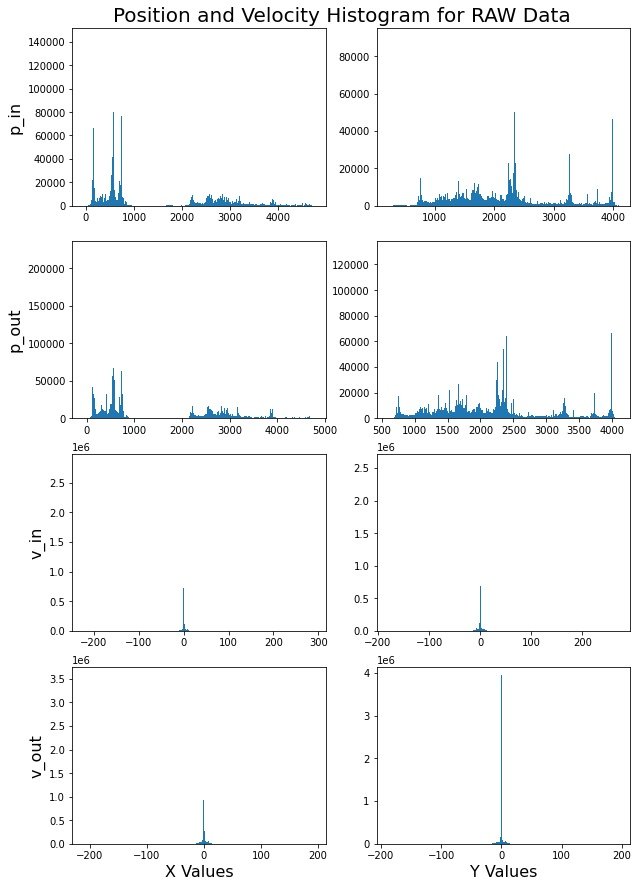
\includegraphics[scale=0.6]{pv_in_out_hist_raw.jpg}
  \caption{Histogram of raw dataset values. Rows from top to bottom: p\_in, p\_out, v\_in, v\_out. Columns from left to right: $x$ values, $y$ values.}
\end{figure}

\begin{figure}
  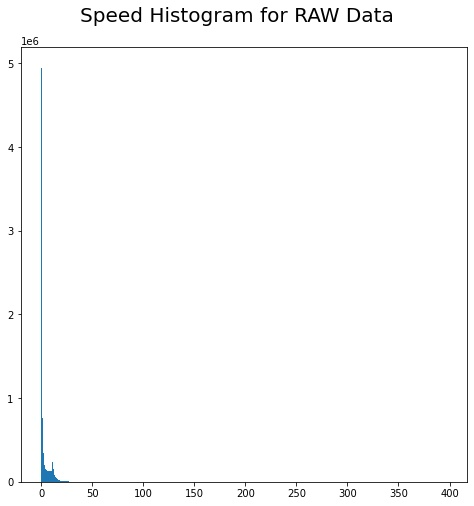
\includegraphics[scale=0.6]{speed_hist.jpg}
  \caption{Speed histogram of raw data for all objects in scenes.}
\end{figure}

\begin{figure}
\hspace*{-1cm} 
  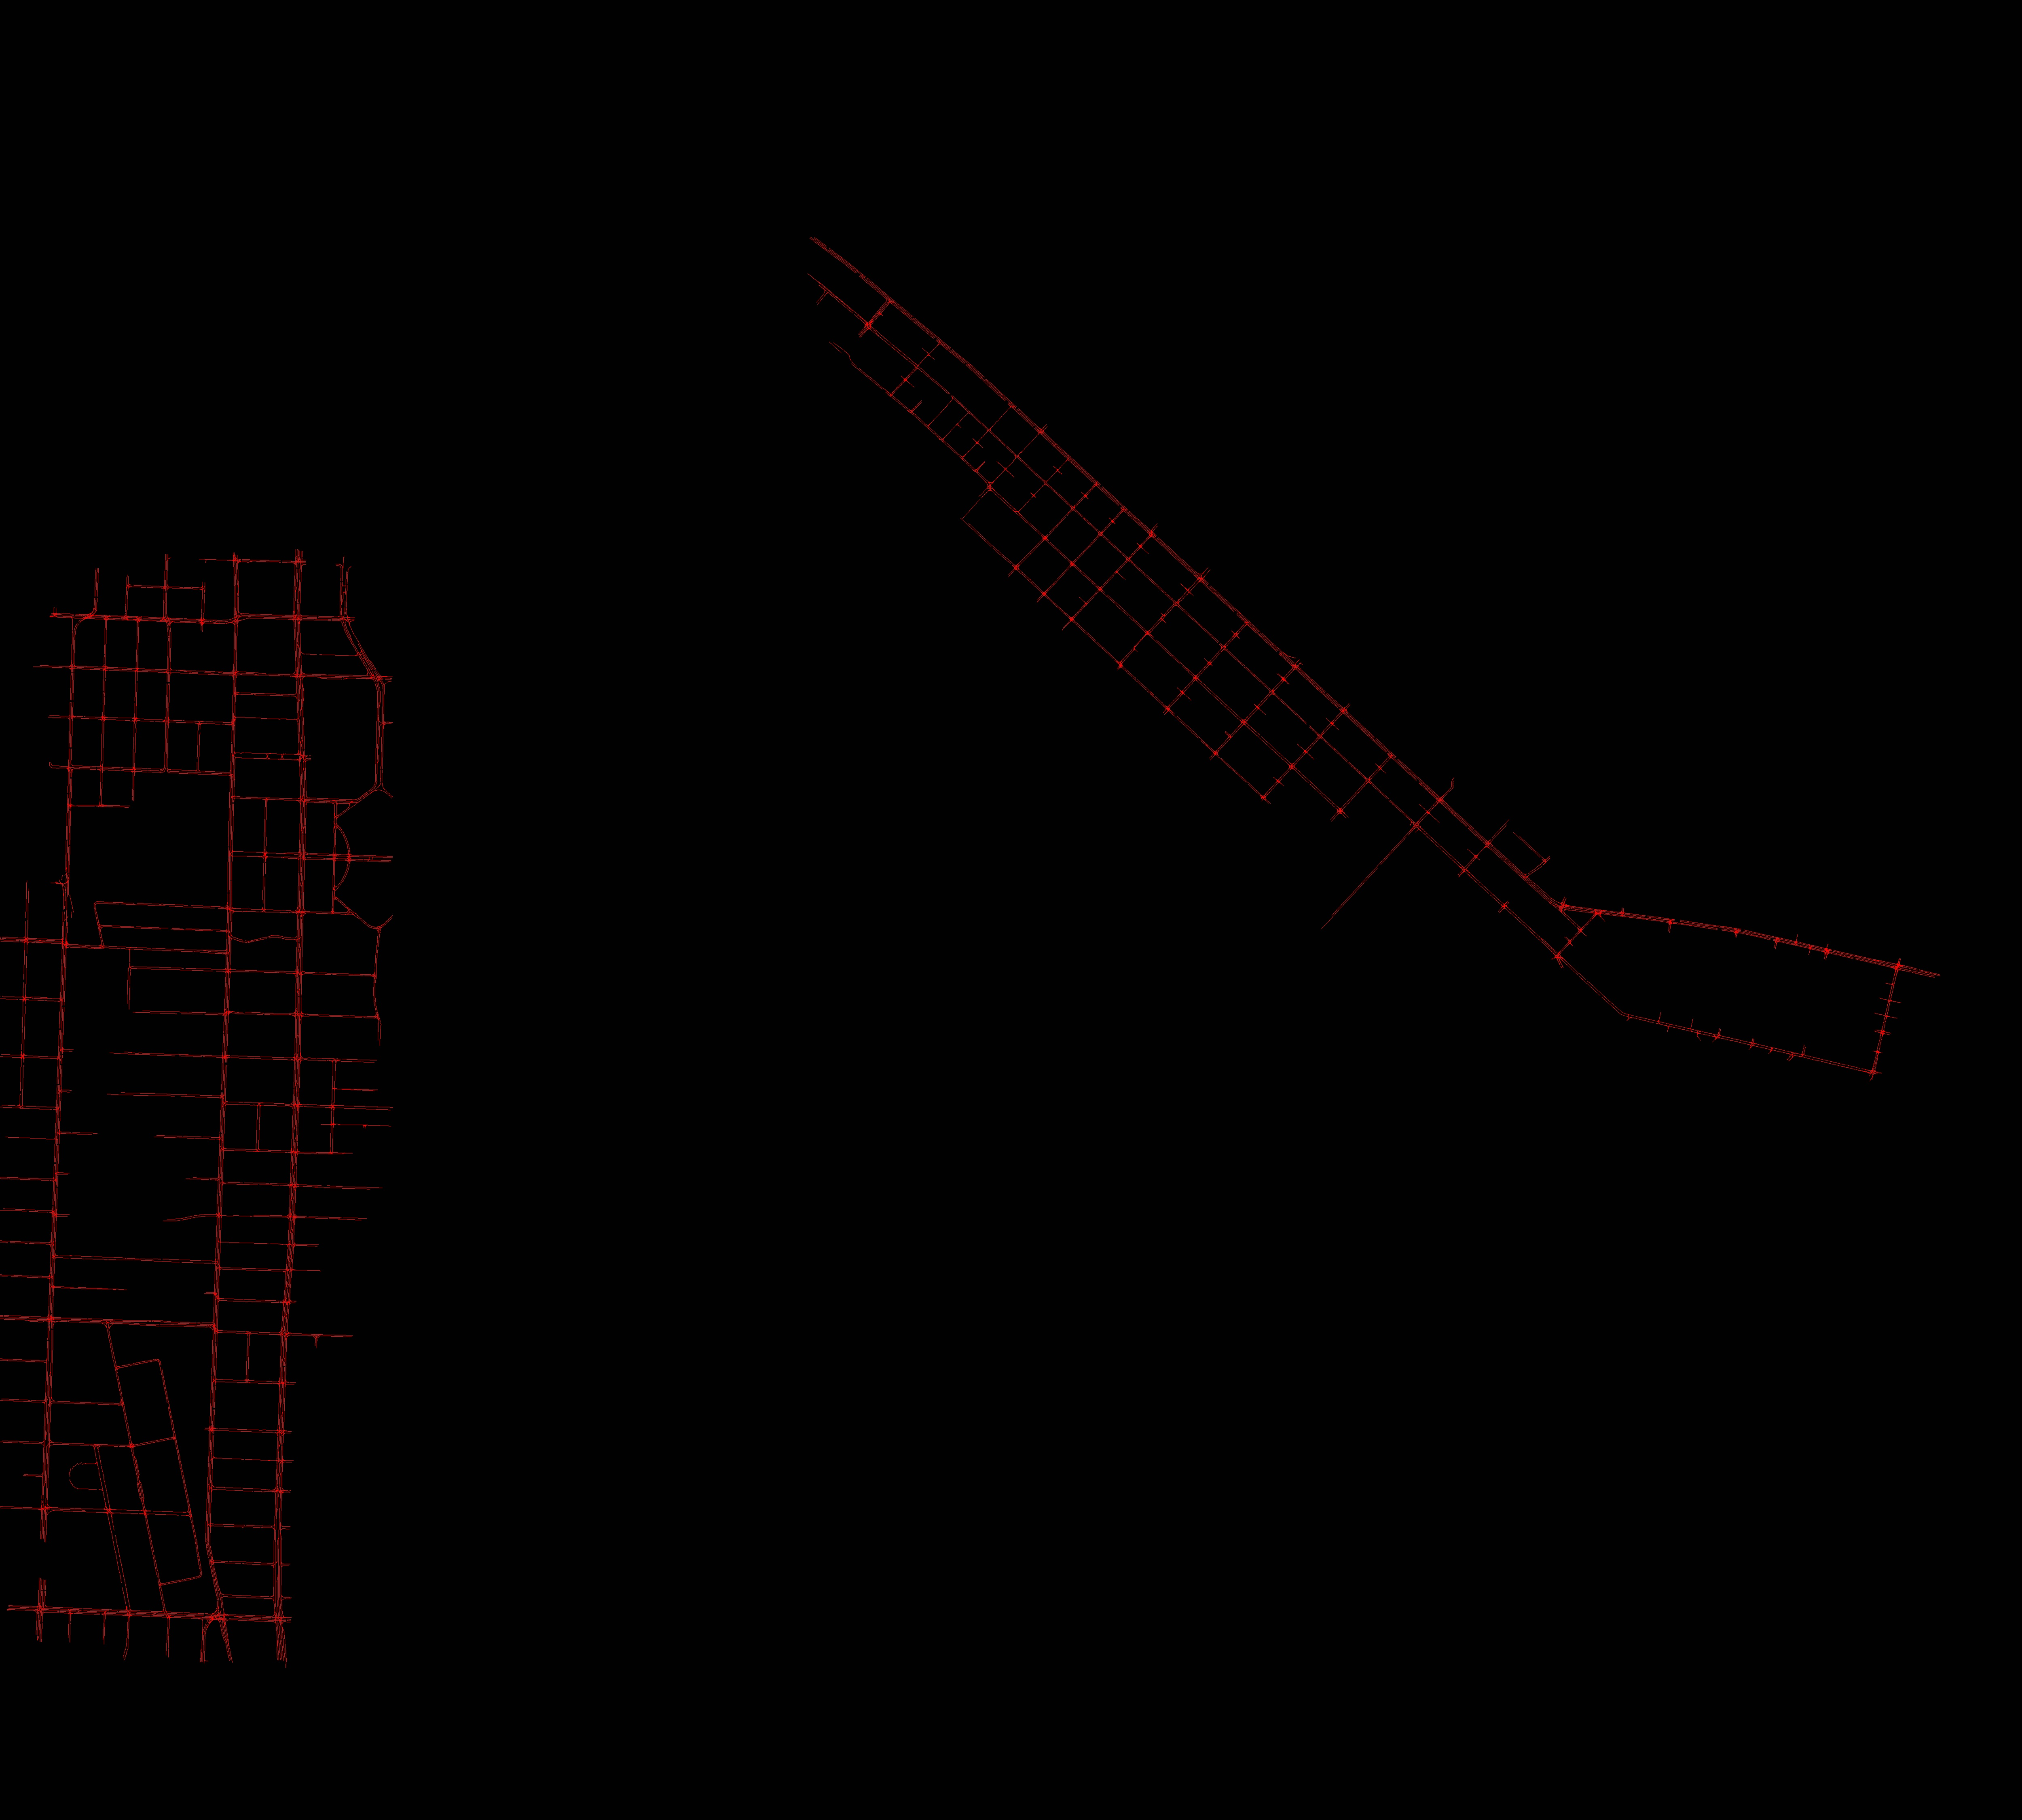
\includegraphics[scale=0.09]{city_map.jpg}
  \caption{A map of the coordinate system with lane information.}
\end{figure}

\begin{figure}
\hspace*{-1cm} 
  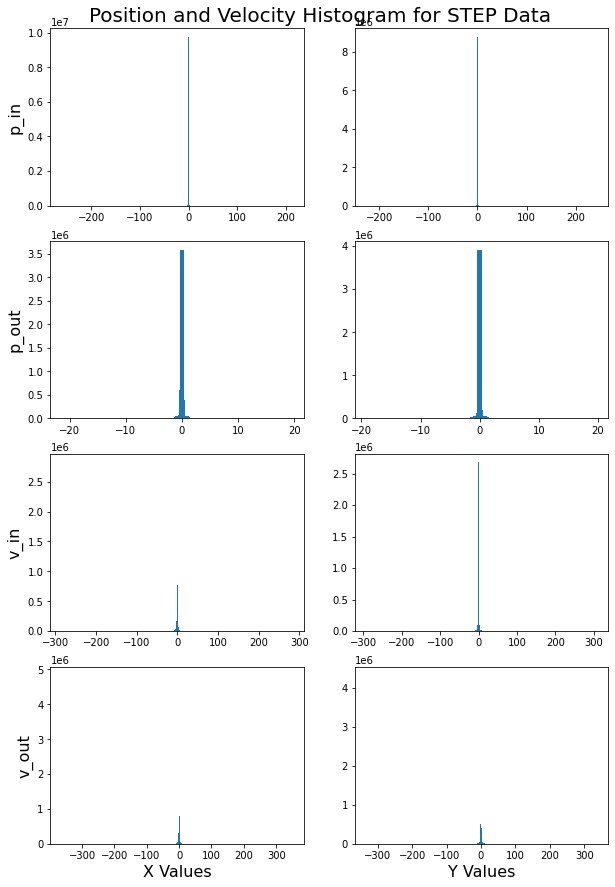
\includegraphics[scale=0.6]{pv_in_out_hist_step.jpg}
  \caption{Histogram of step dataset values. Rows from top to bottom: p\_in, p\_out, v\_in, v\_out. Columns from left to right: $x$ values, $y$ values.}
\end{figure}

\begin{figure}
  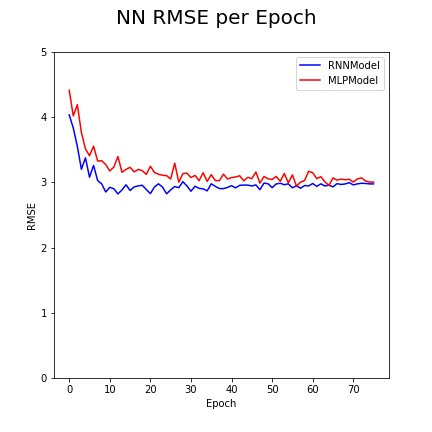
\includegraphics[scale=0.6]{nn_rmse.jpg}
  \caption{The RMSE of the neural network models over time.}
\end{figure}

\begin{changemargin}{-7cm}{-6cm}
\setlength{\voffset}{-0.75in}
\setlength{\headsep}{5pt}
\begin{minipage}{\linewidth}
\centering
  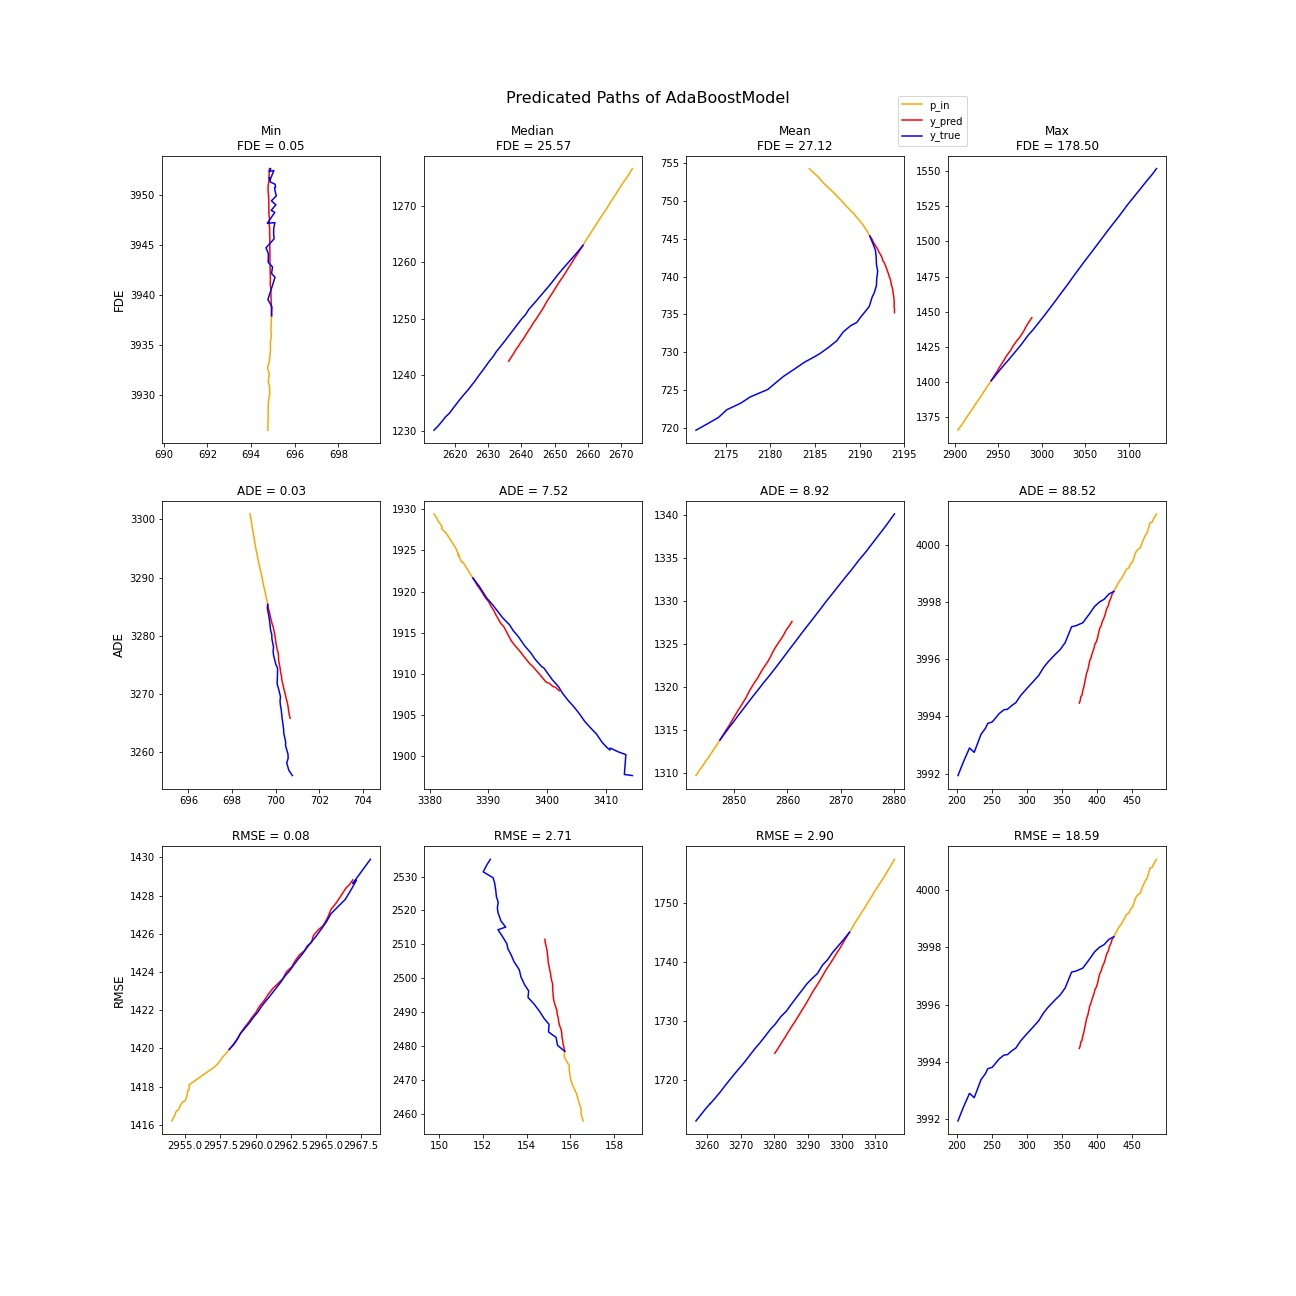
\includegraphics[scale=0.5]{AdaBoostModel_car_paths.jpg}
\end{minipage}
\end{changemargin}

\end{document}